% Overall workflow: logic, decisions and handoffs, with only two named methods.
% Build in Paper/Figure with pdflatex workflow.tex.
\documentclass[tikz,border=3pt]{standalone}
\usepackage{newtxtext,newtxmath}
\usetikzlibrary{arrows.meta,positioning,shapes.arrows,shadows}
% Shared colours for the TikZ schematics; same roles and hex values as
% Code/figures_matlab/paper_style.m (mycolor.space, base #1E5F74).
%   water (P, I, M, W-bar)  teal   | vegetation (V, r, d)  green
%   wind and sand (E, S)    brown  | highlight             orange
%   limits and caps         red dashed
\definecolor{pWater}{HTML}{1E5F74}
\definecolor{pWaterMid}{HTML}{659FB6}
\definecolor{pWaterLight}{HTML}{DCEBF1}
\definecolor{pTeal}{HTML}{00828C}
\definecolor{pVeg}{HTML}{2B633C}
\definecolor{pVegMid}{HTML}{4AC087}
\definecolor{pVegLight}{HTML}{E3F3E8}
\definecolor{pSand}{HTML}{8F7159}
\definecolor{pSandLight}{HTML}{FFEACE}
\definecolor{pAccent}{HTML}{F49431}
\definecolor{pPV}{HTML}{D47216}
\definecolor{pPVLight}{HTML}{FDF1E3}
\definecolor{pPlum}{HTML}{7A437F}
\definecolor{pPlumLight}{HTML}{F2EBF3}
\definecolor{pLimit}{HTML}{D03B3B}
\definecolor{pInk}{HTML}{1F2B33}
\definecolor{pAxis}{HTML}{344A53}
\definecolor{pGrey}{HTML}{97AFB9}
\definecolor{pGreyDark}{HTML}{647B84}
\definecolor{pGrid}{HTML}{E6EBED}

\tikzset{
  tab/.style={rounded corners=4pt, fill=#1, draw=none},
  panel/.style={rounded corners=4pt, draw=#1!70, fill=#1!4, line width=0.7pt},
  question/.style={font=\small\bfseries, text=#1, anchor=west},
  step/.style={rounded corners=3pt, draw=#1!60, fill=white, line width=0.7pt,
    text=pInk, font=\footnotesize, align=center, text width=4.15cm,
    minimum height=1.02cm, inner sep=3pt, drop shadow={opacity=0.12, shadow xshift=0.6pt, shadow yshift=-0.6pt}},
  result/.style={step=#1, fill=#1, draw=#1, text=white, font=\footnotesize\bfseries},
  num/.style={circle, fill=#1, text=white, font=\tiny\bfseries, inner sep=0pt, minimum size=9pt},
  note/.style={font=\footnotesize\itshape, text=pInk, align=left, anchor=west, text width=13.6cm},
  arrow/.style={-{Stealth[length=5.5pt,width=4.5pt]}, draw=#1, line width=1.1pt},
  down/.style={single arrow, fill=#1, draw=none, rotate=-90, minimum height=0.62cm,
    minimum width=0.62cm, single arrow head extend=0.12cm, inner sep=0pt},
  pill/.style={rounded corners=5pt, fill=white, draw=#1, line width=0.6pt, text=#1,
    font=\scriptsize\bfseries, inner xsep=5pt, inner ysep=1.6pt, anchor=west},
}
% \taskrow{y-top}{colour}{task no}{verb}{question}{step1}{step2}{result}{note label}{note}
\newcommand{\taskrow}[9]{%
  \def\yt{#1}%
  \fill[tab=#2] (0,\yt) rectangle (2.05,\yt-2.45);
  \node[text=white, font=\scriptsize\bfseries, align=center] at (1.025,\yt-0.80) {TASK #3};
  \node[text=white, font=\small\bfseries, align=center] at (1.025,\yt-1.35) {#4};
  \draw[panel=#2] (2.20,\yt) rectangle (16.5,\yt-2.45);
  \node[question=#2] at (2.42,\yt-0.30) {#5};
  \node[step=#2] (s1) at (4.62,\yt-1.20) {#6};
  \node[step=#2] (s2) at (9.35,\yt-1.20) {#7};
  \node[result=#2] (s3) at (14.08,\yt-1.20) {#8};
  \node[num=#2] at (s1.north west) {1};
  \node[num=#2] at (s2.north west) {2};
  \draw[arrow=#2] (s1) -- (s2);
  \draw[arrow=#2] (s2) -- (s3);
  \fill[#2] (2.48,\yt-2.17) rectangle (2.56,\yt-1.93);
  \node[note] at (2.62,\yt-2.05) {#9};
}
\begin{document}
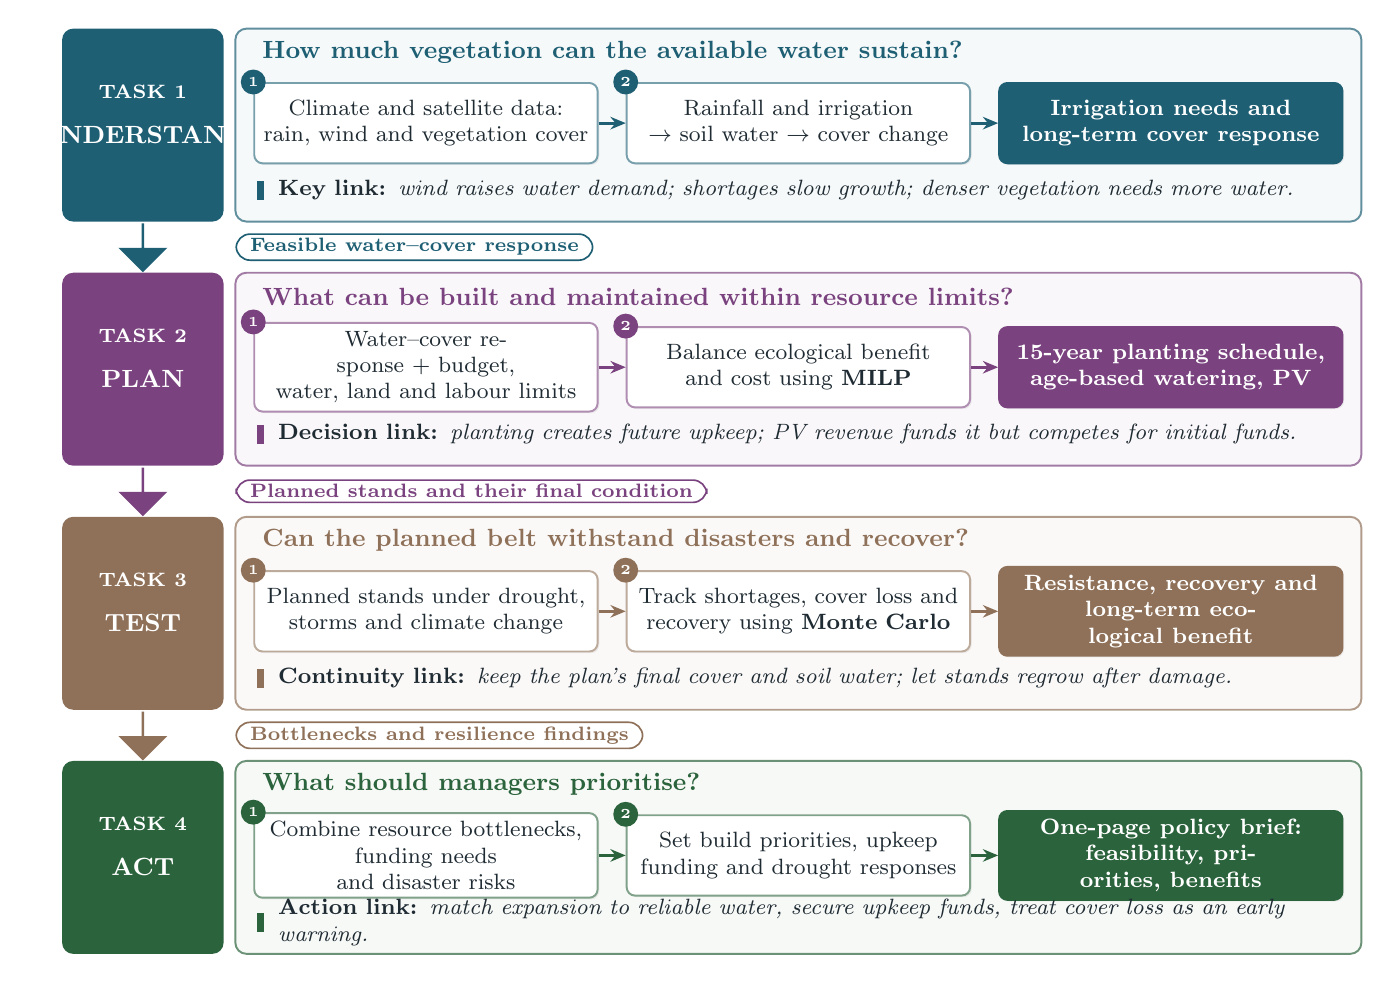
\begin{tikzpicture}
\taskrow{0}{pWater}{1}{UNDERSTAND}
  {How much vegetation can the available water sustain?}
  {Climate and satellite data:\\rain, wind and vegetation cover}
  {Rainfall and irrigation\\$\rightarrow$ soil water $\rightarrow$ cover change}
  {Irrigation needs and\\long-term cover response}
  {\textbf{\upshape Key link:} wind raises water demand; shortages slow growth; denser vegetation needs more water.}

\taskrow{-3.10}{pPlum}{2}{PLAN}
  {What can be built and maintained within resource limits?}
  {Water--cover response $+$ budget,\\water, land and labour limits}
  {Balance ecological benefit\\and cost using \textbf{MILP}}
  {15-year planting schedule,\\age-based watering, PV}
  {\textbf{\upshape Decision link:} planting creates future upkeep; PV revenue funds it but competes for initial funds.}

\taskrow{-6.20}{pSand}{3}{TEST}
  {Can the planned belt withstand disasters and recover?}
  {Planned stands under drought,\\storms and climate change}
  {Track shortages, cover loss and\\recovery using \textbf{Monte Carlo}}
  {Resistance, recovery and\\long-term ecological benefit}
  {\textbf{\upshape Continuity link:} keep the plan's final cover and soil water; let stands regrow after damage.}

\taskrow{-9.30}{pVeg}{4}{ACT}
  {What should managers prioritise?}
  {Combine resource bottlenecks,\\funding needs and disaster risks}
  {Set build priorities, upkeep\\funding and drought responses}
  {One-page policy brief:\\feasibility, priorities, benefits}
  {\textbf{\upshape Action link:} match expansion to reliable water, secure upkeep funds, treat cover loss as an early warning.}

% handoffs between tasks
\foreach \y/\c/\d/\t in {-2.45/pWater/pPlum/{Feasible water--cover response},
                          -5.55/pPlum/pSand/{Planned stands and their final condition},
                          -8.65/pSand/pVeg/{Bottlenecks and resilience findings}} {
  \node[down=\c] at (1.025,\y-0.325) {};
  \node[pill=\c] at (2.20,\y-0.325) {\t};
}
\end{tikzpicture}
\end{document}
